
\chapter{Grundlagen} \index{Grundlagen}

Im ersten Kapitel wird erläutert, was LLM-Tools sind, wie sie trainiert werden und wie sie funktionieren. 
Anschließend werden die einzelnen Tools, die in dieser Arbeit betrachtet werden, vorgestellt und deren 
Entwicklung beschrieben.

Im zweiten Teil des Kapitels wird auf die einzelnen Dokumente, die während des Software-Engineering-Prozesses 
erstellt werden, näher eingegangen und es wird festgelegt, welche Dokumente und Abschnitte in der Analyse betrachtet 
werden. Da sich die Arbeit bei der Erstellung der Dokumente an das Modul ``Secure Software Engineering'' orientiert, 
werden einige Kapitel und Abschnitte nicht betrachtet. Daher wird bei der Beschreibung der entsprechenden Abschnitte ohne 
weitere Begründung erwähnt, dass diese im Folgenden nicht weiter betrachtet werden. Der Vollständigkeit halber werden 
diese aber trotzdem hier im Grundlagenkapitel aufgelistet.

\section{LLM Tools} \index{LLM Tools} \label{LLM Tools}

Unter LLM-Tools versteht man Sprachmodelle, die auf einem Large Language Model (LLM) basieren. Ein LLM ist ein 
Deep-Learning-Algorithmus, der mit sehr großen Datensätzen trainiert wird. Diese Modelle finden häufig Anwendung 
im Bereich des Natural Language Processing (NLP), wo sie verwendet werden, um Abfragen in natürlicher Sprache zu 
beantworten oder Ergebnisse zu liefern. LLMs können neue Inhalte verstehen, zusammenfassen, generieren und vorhersagen. 
Durch das Training sammeln LLMs Milliarden von Parametern, bei denen es sich um Variablen handelt, die im Modell angepasst 
werden, um neue Inhalte abzuleiten.

LLMs basieren auf einem Transformer-Modell, das Eingaben in Token umwandelt und dann gleichzeitig mathematische 
Gleichungen ausführt, um Beziehungen zwischen den Token zu ermitteln. Dadurch kann der Computer Muster erkennen, 
die auch ein Mensch wahrnehmen würde, wenn ihm die gleiche Frage gestellt wird. Zudem verwenden Transformer-Modelle 
Selbstaufmerksamkeitsmechanismen, die es dem Modell ermöglichen, schneller zu lernen als herkömmliche Modelle. Somit 
kann das Transformer-Modell verschiedene Teile der Sequenz oder den gesamten Kontext eines Satzes berücksichtigen, um 
Vorhersagen zu generieren.

Grundsätzlich bestehen LLMs aus vier neuronalen Netzwerkschichten: der wiederkehrenden Ebene, der Einbettungsebene, 
der Feedforward-Ebene und der Aufmerksamkeitsebene. Diese Schichten arbeiten zusammen, um den Eingabetext zu 
verarbeiten und Ausgabeinhalte zu generieren.\\
Die wiederkehrende Ebene dient dazu, die Wörter des Eingabetextes der Reihe nach zu interpretieren und die 
Beziehungen zwischen den Wörtern in einem Satz zu erfassen. Die Einbettungsebene erfasst die semantische und 
syntaktische Bedeutung der Eingabe, sodass das Modell den Kontext verstehen kann. Die Feedforward-Schicht besteht 
aus mehreren vollständig verbundenen Schichten, die die Eingabeeinbettungen transformieren. Dadurch ermöglichen 
diese Schichten dem Modell, Abstraktionen auf höherer Ebene zu verstehen und somit die Absicht des Benutzers mit 
der Texteingabe zu erfassen. Die Aufmerksamkeitsebene ermöglicht es dem Sprachmodell, sich auf einzelne Teile des 
Eingabetextes zu konzentrieren, die für die Aufgabe relevant sind, und dadurch die genausten Ausgaben zu generieren.

Damit ein großes Sprachmodell Texteingaben empfangen und eine Ausgabevorhersage generieren kann, muss es zunächst 
allgemein geschult und anschließend feinabgestimmt werden, um spezifische Aufgaben ausführen zu können. Für die 
Schulung werden riesige Datenmengen im Petabyte-Bereich benötigt. Das Training verläuft mehrstufig und beginnt 
in der Regel mit einem unbeaufsichtigten Lernansatz, bei dem das Modell mit unstrukturierten und unbeschrifteten 
Daten trainiert wird, da diese in größeren Mengen verfügbar sind. In dieser Phase leitet das Modell Beziehungen 
zwischen verschiedenen Wörtern und Konzepten ab.\\
Anschließend erfolgt die Schulung und Feinabstimmung durch eine Form des selbstüberwachten Lernens. Dabei wird 
eine Datenkennzeichnung durchgeführt, durch die das Modell verschiedene Konzepte besser und genauer identifizieren 
kann. Im nächsten Schritt durchläuft das LLM den Transformationsprozess im Rahmen des Deep Learning. Die 
Transformer-Modellarchitektur ermöglicht es dem LLM, mittels eines Selbstaufmerksamkeitsmechanismus Beziehungen 
und Verbindungen zwischen Wörtern und Konzepten zu erkennen, indem bestimmten Elementen (Token) Bewertungen 
zugewiesen werden, um die Beziehungen festzulegen.


Entscheidend für die Leistungsfähigkeit und die Qualität eines Sprachmodells sind die Datensätze, die zum 
Trainieren verwendet werden \cite{GrundlagenLLM}. Daher wird im weiteren mit drei unterschiedlichen LLM Tools gearbeitet, auf die 
in den folgenden Abschnitten einzeln eingegangen wird. 

\subsection{ChatGPT} \index{ChatGPT} \label{ChatGPT}


ChatGPT wurde von OpenAI am 30. November 2022 veröffentlicht und entwickelte sich aufgrund seiner fortschrittlichen 
generativen KI-Fähigkeiten rasch zu einer internationalen Sensation. Wenn man ChatGPT fragt, ob es einen Infotext 
zu sich selbst erstellen kann, erhält man die Antwort in \autoref{InfotextChatGPT}.

\begin{prompt} 
    \begin{tcolorbox}[colback=gray!20, colframe=gray!20, boxrule=0pt, sharp corners] 
    \textbf{Prompt: Erstell mir einen Infotext über dich für meine Bachelorarbeit}

    ChatGPT ist ein fortschrittlicher KI-gestützter Sprachassistent, der auf der GPT-4-Architektur von OpenAI basiert. 
    Entwickelt im Rahmen der Forschung und Entwicklung im Bereich Künstliche Intelligenz, ist ChatGPT in der Lage, 
    natürliche Sprache zu verstehen und darauf zu antworten. Dies macht ihn zu einem vielseitigen Werkzeug für eine 
    Vielzahl von Anwendungen, von der Beantwortung alltäglicher Fragen bis hin zur Unterstützung bei komplexeren 
    Aufgaben wie dem Schreiben von Texten, der Generierung von Ideen und der Bereitstellung von Informationen.
    
    Die GPT-4-Architektur, auf der ChatGPT basiert, verwendet tiefes maschinelles Lernen, um menschliche Sprache zu 
    verarbeiten und zu erzeugen. Durch die Analyse großer Mengen an Textdaten kann das Modell Muster und Zusammenhänge 
    erkennen, die es ihm ermöglichen, kontextuell relevante und kohärente Antworten zu geben. Diese Fähigkeiten machen 
    ChatGPT zu einem nützlichen Instrument in Bereichen wie Bildung, Forschung, Kundenservice und mehr.
    
    Ein weiterer bemerkenswerter Aspekt von ChatGPT ist seine Fähigkeit, sich an eine Vielzahl von Themen anzupassen 
    und Informationen auf klare und präzise Weise zu vermitteln. Dies wird durch kontinuierliches Training und 
    Verbesserung des Modells erreicht, wobei sowohl technische Fortschritte als auch Nutzerfeedback berücksichtigt 
    werden.
    
    Zusammengefasst ist ChatGPT ein leistungsstarker und vielseitiger KI-Assistent, der durch seine fortschrittliche 
    Technologie und seine breite Anwendbarkeit einen wertvollen Beitrag in vielen Bereichen leistet.
    \vfill
    \end{tcolorbox}
    \caption{Infotext ChatGPT, Quelle: ChatGPT}
    \label{InfotextChatGPT}
\end{prompt}

Die Beta-Version der Plattform war zunächst kostenlos verfügbar, und OpenAI bot den Nutzern weiterhin eine kostenlose 
Basisversion an. Im Februar 2023 führte OpenAI ein kostenpflichtiges Abonnement ein, das unbegrenzten Zugriff auf ChatGPT 
sowie eine erweiterte Palette von Funktionen und Diensten ermöglichte.

Trotz der begeisterten Resonanz löste ChatGPT auch einige Kontroversen aus. Es lieferte teilweise fehlerhafte Antworten, 
insbesondere bei Aufgaben wie Schlussfolgerungen ziehen, Nuancen analysieren, Meinungen bewerten oder Vorhersagen treffen. 
Pädagogen weltweit äußerten Bedenken hinsichtlich des Einsatzes von ChatGPT im Bildungsbereich, auch an Universitäten wurde 
der Einsatz kritisch diskutiert.

Trotz dieser Kontroversen schien ChatGPT bereit zu sein, die Erstellung von Inhalten im Internet zu revolutionieren. 
Webentwickler und Content-Ersteller nutzten ChatGPT zunehmend als Recherche- und Schreibhilfe für Website-Texte.

Im März 2023 brachte OpenAI eine neue Version heraus, bekannt als GPT-4. Ein bedeutender Unterschied zu früheren Versionen 
bestand darin, dass GPT-4 Eingaben sowohl in Text- als auch in Bildformaten akzeptierte. Dies ermöglichte dem Chatbot, Daten 
aus Diagrammen, Grafiken und Screenshots zu interpretieren. Zudem machte GPT-4 deutlich weniger Denkfehler und sachliche Fehler, 
auch ``Halluzinationen'' genannt, als das zuvor verwendete GPT-3.5-Modell. Am Ende des Jahres hatte sich ChatGPT weiterentwickelt 
und konnte beispielsweise Bilder analysieren, Sprachansagen verarbeiten und gesprochene Antworten geben.

Im Mai 2024 kündigte OpenAI ein aktualisiertes Modell namens ChatGPT-4o an, das schnellere Ergebnisse sowie verbesserte 
Text- und Audiofunktionen versprach. Dieses Modell umfasst auch ein neues Konversations-KI-System namens ``Sky'' \cite{GrundlagenChatGPT}.

\subsection{Google Gemini} \index{Google Gemini} \label{Google Gemini}

Im Dezember 2023 stellte Google eine generative Künstliche Intelligenz mit dem Namen Google Gemini vor. Sie wurde von Google DeepMind 
entwickelt und ist laut Aussage von Google das größte, leistungsstärkste und vielseitigste große Sprachmodell (LLM), das bisher von 
Google entwickelt und realisiert wurde. In der ursprünglichen Ankündigung wurde das KI-Sprachmodell unter dem Namen Gemini vorgestellt. 
Im Februar 2024 entschied Google, auch den bisher als Bard bekannten Chatbot in Gemini umzubenennen. Damit ist Gemini mittlerweile sowohl
der Name des Google Chatbot als auch des zugrundeliegenden Sprachmodells.

Bei Nachfrage an Gemini, ob es einen Infotext über sich erstellen kann, erhält man die Antwort in \autoref{InfotextGemini1} und \autoref{InfotextGemini2}.

\begin{prompt}
    \begin{tcolorbox}[colback=gray!20, colframe=gray!20, boxrule=0pt, sharp corners] 
    \textbf{Prompt: Erstell mir einen Infotext über dich für meine Bachelorarbeit}\\ 
        \textbf{Was ist Gemini?}\\
        Gemini ist ein Large Language Model (LLM) von Google AI, das mit einem riesigen Datensatz aus Text und Code 
        trainiert wurde. Es kann Text generieren, Sprachen übersetzen, verschiedene Arten von kreativen Inhalten schreiben 
        und Ihre Fragen auf informative Weise beantworten. Gemini befindet sich noch in der Entwicklung, hat aber bereits gelernt,
        viele Arten von Aufgaben auszuführen, einschließlich:
        \begin{itemize}
            \item Befolgen Sie Anweisungen und erledigen Sie Aufgaben sorgfältig.
            \item Beantworten Sie Ihre Fragen umfassend und informativ, auch wenn sie offen, herausfordernd oder seltsam sind.
            \item Generieren Sie verschiedene kreative Textformate, wie Gedichte, Codes, Skripte, Musikstücke, E-Mails, Briefe usw. 
                  Ich werde mein Bestes tun, um alle Ihre Anforderungen zu erfüllen.
        \end{itemize}
        \textbf{Technische Details}\\
        Gemini basiert auf der Transformer-Architektur und wird mit einem massiven Datensatz aus Text und Code trainiert. 
        Es verwendet eine Vielzahl von Techniken, um seine Leistung zu verbessern, einschließlich:
        \begin{itemize}
            \item \textbf{Aufmerksamkeit:} Ermöglicht es Gemini, sich auf die relevantesten Teile einer Eingabe zu konzentrieren.
            \item \textbf{Beam Search:} Ermöglicht Gemini, die besten möglichen Ausgaben zu generieren.
            \item \textbf{Multitasking:} Ermöglicht Gemini, mehrere Aufgaben gleichzeitig zu lernen und auszuführen.
        \end{itemize}
        \textbf{Anwendungen}\\
        Gemini kann für eine Vielzahl von Anwendungen eingesetzt werden, einschließlich:
        \begin{itemize}
            \item \textbf{Generierung von kreativen Inhalten:} Gemini kann verwendet werden, um Gedichte, Codes, Skripte, Musikstücke, 
            E-Mails, Briefe usw. zu generieren.
            \item \textbf{Sprachübersetzung:} Gemini kann verwendet werden, um Text von einer Sprache in eine andere zu übersetzen.
            \item \textbf{Beantwortung von Fragen:} Gemini kann verwendet werden, um Ihre Fragen umfassend und informativ zu beantworten, 
            auch wenn sie offen, herausfordernd oder seltsam sind.
            \item \textbf{Zusammenfassen von Texten:} Gemini kann verwendet werden, um lange Textpassagen zu zusammenfassen.
            \item \textbf{Schreiben verschiedener Arten von kreativen Textformaten:} Gemini kann verwendet werden, um verschiedene Arten von 
            kreativen Textformaten zu schreiben, wie Gedichte, Codes, Skripte, Musikstücke, E-Mails, Briefe usw.
        \end{itemize}
    \vfill
    \end{tcolorbox}
    \caption{Infotext Gemini 1, Quelle: Gemini}
    \label{InfotextGemini1}
\end{prompt}

\begin{prompt} 
    \begin{tcolorbox}[colback=gray!20, colframe=gray!20, boxrule=0pt, sharp corners] 
        \textbf{Ethische Überlegungen}\\
        Es ist wichtig, Gemini verantwortungsvoll und ethisch zu nutzen. Zu den ethischen Überlegungen, die bei der Verwendung von Gemini zu beachten sind, gehören:
        \begin{itemize}
            \item \textbf{Vermeidung von Vorurteilen:} Gemini wird mit einem riesigen Datensatz aus Text und Code trainiert. Dieser Datensatz 
            kann Vorurteile enthalten, die sich in den Ausgaben von Gemini widerspiegeln können. Es ist wichtig, sich dieser Vorurteile bewusst 
            zu sein und Maßnahmen zu ergreifen, um sie zu mindern.
            \item \textbf{Vermeidung von Schadenszufügung:} Gemini kann verwendet werden, um schädlichen Text zu generieren, z. B. Hassreden 
            oder Gewaltandrohungen. Es ist wichtig, Gemini nicht zu verwenden, um anderen Schaden zuzufügen.
            \item \textbf{Respekt vor der Privatsphäre:} Gemini kann verwendet werden, um personenbezogene Daten zu generieren. Es ist wichtig, 
            Gemini nicht zu verwenden, um die Privatsphäre anderer zu verletzen.
        \end{itemize}
        \textbf{Fazit}\\
        Gemini ist ein leistungsstarkes Tool, das für eine Vielzahl von Anwendungen eingesetzt werden kann. Es ist jedoch wichtig, Gemini verantwortungsvoll und ethisch zu nutzen.
    \vfill
    \end{tcolorbox}
    %\addtocounter{figure}{-1}
    \caption{Infotext Gemini 2, Quelle: Gemini}
    \label{InfotextGemini2}
\end{prompt}

Gemini 1.0 wurde in drei verschiedenen Größen optimiert: Gemini Ultra als das größte und leistungsstärkste Modell 
für hochkomplexe Aufgaben, Gemini Pro als das beste Modell zur Anwendung in einem breiten Aufgabenspektrum und Gemini 
Nano als das effizienteste Modell für Aufgaben, die direkt auf dem Gerät verarbeitet werden.

Die Gemini-Modelle sind von Grund auf multimodal konzipiert, was bedeutet, dass sie mit verschiedenen Arten von 
Informationen umgehen können. Gemini ist in der Lage, Texte, Programmcode, Bilder, Videos, Audioinformationen und 
deren Kombinationen zu analysieren, zu verstehen, zu kombinieren und zu generieren. Da Gemini auch mit Skizzen und 
handgeschriebenem Text umgehen kann, eignet es sich für den Einsatz in Fachbereichen wie zum Beispiel Mathematik oder Physik. 
Im Programmierbereich werden gängige Programmiersprachen wie Python, Java, C++ oder Go unterstützt. Gemini 
kann Programmcode analysieren, kommentieren und auch generieren. Dadurch steht Gemini in Konkurrenz zu anderen LLMs 
wie den GPT-Sprachmodellen von Open AI. Gemini soll jedoch die Konkurrenzprodukte in vielen Benchmarks deutlich übertreffen.

Gemini baut auf den ebenfalls von Google entwickelten Sprachmodellen LaMDA und PaLM 2 auf. Wie üblich für 
LLMs (Large Language Models) basiert auch Gemini auf einer Transformer-Architektur. Google hat die Architektur des 
Modells zur Skalierung der Trainingsfähigkeiten optimiert und mit einem Multi-Query-Aufmerksamkeitsmechanismus ausgestattet. 
Die unterstützte Kontextlänge beträgt 32.000 Tokens und in der Version 1.5 bis zu einer Million Tokens. Gemini wurde mit 
Daten verschiedener Modalitäten trainiert, und als Trainingsplattform verwendete Google Rechner-Cluster und Tensor 
Processing Units (TPUs) der neuesten Generation v4 und v5 als KI-Beschleuniger.

Google hat begonnen, die KI in zahlreiche eigene Produkte zu integrieren, um die Fähigkeiten der Websuche, des 
Chrome-Browsers, des GMail-Services, verschiedener Entwicklungstools und anderer Produkte und Services zu verbessern 
und zu erweitern. Mitte Februar 2024 stellte Google Gemini 1.5 und 1.5 Pro vor, welche bis zu eine Million Tokens 
verarbeiten können. Diese neuen Versionen sollen die Benchmark-Ergebnisse der Vorgängerversion deutlich übertreffen \cite{GrundlagenGemini}.

\subsection{Le Chat} \index{Le Chat} \label{Le Chat}

\begin{prompt}
    \begin{tcolorbox}[colback=gray!20, colframe=gray!20, boxrule=0pt, sharp corners] 
        \textbf{Prompt: Erstell mir einen Infotext über Le Chat für meine Bachelorarbeit}
        \textbf{Einleitung}\\
        Le Chat ist ein fortschrittliches Sprachmodell, das auf künstlicher Intelligenz (KI) und maschinellem Lernen 
        basiert. Entwickelt von einem Team aus Experten für KI und Sprachverarbeitung, hat Le Chat die Fähigkeit, 
        menschliche Sprache zu verstehen, zu interpretieren und darauf zu reagieren, was es zu einem wertvollen 
        Werkzeug in verschiedenen Branchen macht.

        \textbf{Funktionsweise}\\
        Le Chat nutzt eine Kombination aus Techniken des Natural Language Processing (NLP) und des Deep Learning. NLP 
        ermöglicht es dem Modell, die Struktur und den Kontext der menschlichen Sprache zu verstehen, während Deep 
        Learning-Algorithmen verwendet werden, um Muster in den Daten zu erkennen und die Genauigkeit der Vorhersagen 
        zu verbessern.

        \textbf{Anwendungsbereiche}\\
        Le Chat kann in einer Vielzahl von Anwendungen eingesetzt werden. Einige der wichtigsten Anwendungsbereiche sind:
        \begin{itemize}
            \item \textbf{Kundenservice:} Le Chat kann als virtueller Assistent eingesetzt werden, um Kundenanfragen zu 
            beantworten, Produktempfehlungen auszusprechen und den Kunden bei der Lösung von Problemen zu unterstützen.
            \item \textbf{Bildung:} Le Chat kann als Tutor-System eingesetzt werden, um Schülern und Studenten bei der 
            Lösung von Aufgaben und beim Verständnis von komplexen Konzepten zu helfen.
            \item \textbf{Gesundheitswesen:} Le Chat kann als virtueller Gesundheitsassistent eingesetzt werden, um 
            Patienten bei der Verwaltung ihrer Medikamente zu unterstützen, Gesundheitstipps zu geben und in Notfällen 
            Erste Hilfe-Anweisungen bereitzustellen.
            \end{itemize}
        \textbf{Vorteile}\\
        Le Chat bietet eine Reihe von Vorteilen gegenüber herkömmlichen Sprachmodellen. Einige der wichtigsten Vorteile sind:
        \begin{itemize}
            \item \textbf{Verbesserte Genauigkeit:} Le Chat nutzt fortschrittliche Deep Learning-Algorithmen, um die 
            Genauigkeit der Vorhersagen zu verbessern und eine bessere Benutzererfahrung zu bieten.
            \item \textbf{Skalierbarkeit:} Le Chat kann leicht skaliert werden, um eine große Anzahl von Anfragen 
            gleichzeitig zu bearbeiten, was es zu einer idealen Lösung für Unternehmen mit hohem Kundenaufkommen macht.
            \item \textbf{Kosteneffizienz:} Le Chat kann als kosteneffiziente Alternative zu menschlichen Kundenservice-Mitarbeitern 
            eingesetzt werden, was zu erheblichen Einsparungen für Unternehmen führen kann.
            \end{itemize}
        \textbf{Fazit}\\
        Le Chat ist ein innovatives Sprachmodell, das die Fähigkeit hat, die Art und Weise, wie wir mit Maschinen 
        interagieren, zu revolutionieren. Mit seiner fortschrittlichen Technologie und seinen vielfältigen 
        Anwendungsmöglichkeiten ist Le Chat ein wichtiger Meilenstein in der Entwicklung der KI und ein Werkzeug, 
        das in Zukunft eine noch größere Rolle spielen wird.
        \vfill
    \end{tcolorbox}
    \caption{Infotext Le Chat, Quelle: Le Chat}
    \label{InfotextLeChat}
\end{prompt}

In \autoref{InfotextLeChat} sieht man die Antwort die Le Chat gibt, wenn man ihn nach einem Infotext über sich 
fragt. Le Chat ist ein, von dem französischem KI-Startup Mistral AI veröffentlichter Chatbot. Mistral AI startete mit  
seinen frei verwendbaren Sprachmodellen, also auf der Grundlage von Open Source, erfolgreich durch. Nun  
hat Mistral AI sein bislang größtes Modell 'Mistral Large' veröffentlicht. Diesmal allerdings nicht auf der  
Basis von Open Source, sondern ausschließlich über die eigene Webseite und der KI-Infrastruktur Microsoft  
Azure. Es lassen sich allerdings API-Keys für Programmierschnittstellen erstellen, um z.B. Mistral Large über  
seinen eigenen Server laufen zu lassen und so für andere User auf der eigenen Homepage verfügbar zu machen.  
Mit Mistral Large wurde auch Le Chat veröffentlicht, welcher aktuell kostenfrei verwendet werden kann.
Le Chat bietet derzeit noch sehr wenige Funktionen an. Es stehen Lediglich Texteingabe und -ausgabe zur Verfügung.  
Die Datengrundlage reicht nur bis 2021, weshalb es auch hier, für die Jahre 2022 bis heute, zu der Problematik der  
Halluzination kommen kann.
Grundsätzlich kann man zwischen drei Sprachmodellen auswählen: Large, Next und Small. Large bietet überlegene Denkfähigkeit,  
Next ist ein Prototyp-Modell für erhöhte Kürze und Small arbeitet schnell und kosteneffektiv \cite{GrundlagenLeChat}.


\section{Software Engineering Prozess}

\begin{figure}
    \centering
    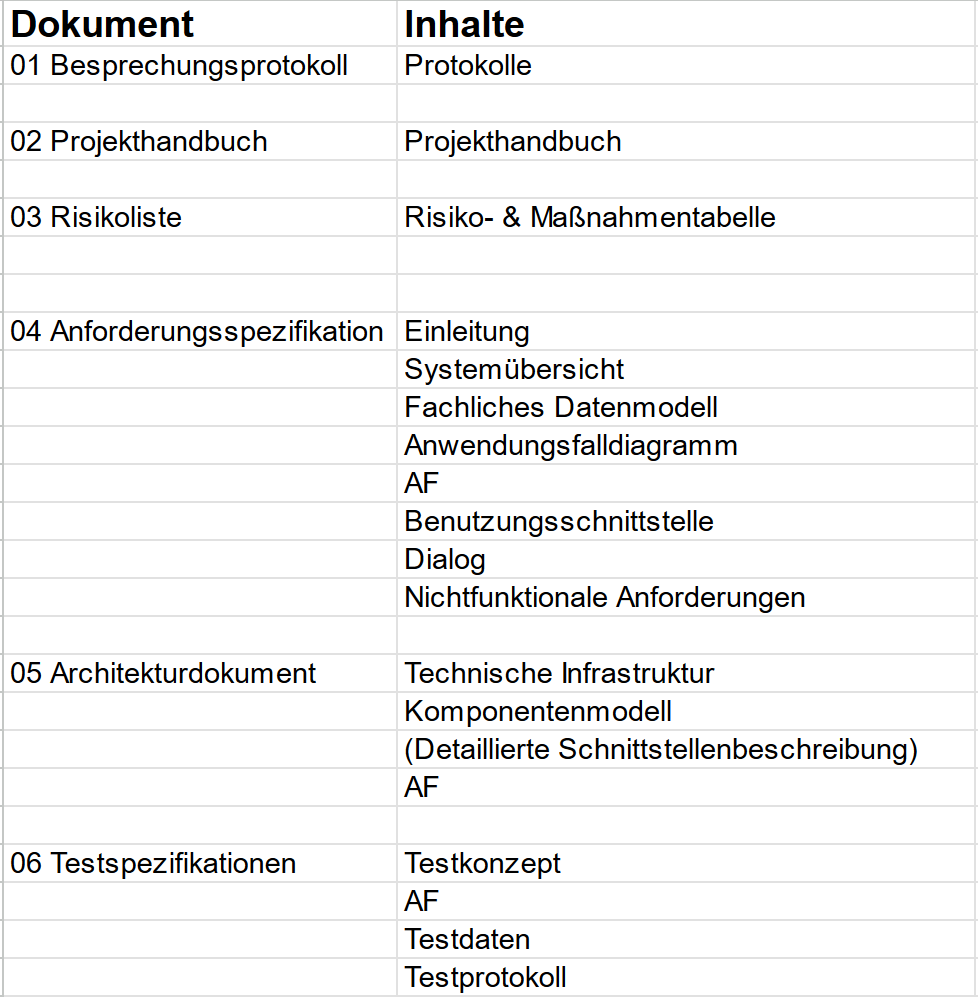
\includegraphics{pictures/TabelleKap2.PNG}
    \caption{Dokumente im Software Engineering}
    \label{Dokumente Software Engineering}
\end{figure}

Software-Engineering ist eine technische Disziplin, die sich umfassend mit der Erstellung von Software beschäftigt, 
beginnend bei der Konzeption, über den Betrieb, bis hin zur Wartung. Die wesentlichen Aktivitäten im 
Software-Engineering umfassen die Softwarespezifikation, -entwicklung, -validierung und -weiterentwicklung 
\cite{Sommerville10}. Während des Prozesses werden mehrere Dokumente erstellt und im Verlauf angepasst. 
Diese umfassen Besprechungsprotokolle, eine Risikoliste, ein Projekthandbuch, eine Anforderungsspezifikation, 
ein Architekturdokument und eine Testspezifikation. In der \autoref{Dokumente Software Engineering} sieht man, 
welche Inhalte die einzelnen Dokumente umfassen. Diese werden im Folgenden etwas genauer beschrieben, um einen 
Überblick über die Dokumente zu vermitteln.

\subsection{Besprechungsprotokoll} \index{Besprechungsprotokoll} \label{Besprechungsprotokoll}

Alle Team- und Kundengespräche werden systematisch in Besprechungsprotokollen dokumentiert. Diese Protokolle enthalten 
Aufträge, Beschlüsse, Feststellungen und Informationen, die in Form von Texten, Bildern, Diagrammen usw. festgehalten 
werden. Aufträge müssen mit einem Fälligkeitsdatum und einem Verantwortlichen versehen sein, während Beschlüsse klar 
und unmissverständlich formuliert werden sollten. Im Rahmen der Anforderungsanalyse werden in Beschlüssen die 
Benutzeranforderungen erfasst. Feststellungen hingegen sind Beschlüsse, die keine Abstimmung benötigen, können 
aber ebenfalls Anforderungen an das System enthalten. Informationen bieten den Projektmitgliedern wichtige Hinweise. 
Dabei ist zu beachten, dass ein Besprechungsprotokoll keine Erlebniserzählung sein soll.

Der Aufbau eines Besprechungsprotokolls gestaltet sich wie folgt: Am Anfang stehen Datum, Thema, Verfasser, 
Teilnehmer und Verteiler. Anschließend wird eine Tabelle mit den Spalten Nummer, Art, Beschreibung, Termin und 
Verantwortlicher erstellt. Die Nummer stellt eine eindeutige ID im Protokoll dar. Die Art spezifiziert, ob es sich 
um einen Auftrag (=A), einen Beschluss (=B), eine Feststellung (=F) oder eine Information (=I) handelt. Die 
Beschreibung fasst den Auftrag, den Beschluss, die Feststellung oder die Information kurz und präzise zusammen. Der 
Termin gibt an, bis wann der Auftrag erledigt sein muss. Der Verantwortliche benennt die Person, die den Auftrag 
ausführen muss, den Beschluss gefasst hat oder die Feststellung bzw. die Information geliefert hat.

\subsection{Projekthandbuch} \index{Projekthandbuch} \label{Projekthandbuch}

Das Projekthandbuch dient dazu, die Projektmitglieder umfassend über das Projekt zu informieren, einschließlich der 
Vorgeschichte, Vertragsbasis, Grundlagen, Ziele, Ergebnisse und mehr. Es bietet zudem eine Übersicht über die 
Projektorganisation, wie z.B. die Teamaufstellung, das Berichtswesen und die Dokumentenablage, sowie über wesentliche 
Projektabläufe wie Änderungsverfahren, Risikomanagement und Aufwandsverfolgung. Ziel des Projekthandbuchs ist es, neuen 
Teammitgliedern den Einstieg zu erleichtern und auf wichtige Dokumente hinzuweisen, die für die Projektabwicklung 
notwendig sind. Damit fungiert das Projekthandbuch als zentrale Anlaufstelle für das Projekt.

Das Dokument beginnt mit einer Einleitung, die die Rahmenbedingungen klärt. Dieser Abschnitt enthält den Zweck des 
Dokuments, Hinweise zur Redaktion, in denen festgelegt wird, wer für das Dokument verantwortlich ist, sowie 
Informationen zum Verteiler, also wer bei Änderungen informiert werden muss.

Im Anschluss folgt die Projektbeschreibung, die die Rahmenbedingungen des Projekts darlegt. Dieser Teil enthält einen 
Abschnitt zur Vorgeschichte, in dem beschrieben wird, wie es zu dem Projekt kam. Ein weiterer Abschnitt bietet eine 
inhaltliche Kurzdarstellung des Projekts. Danach werden in einem Abschnitt zur Vertragsbasis der zeitliche 
Projektrahmen, die Anzahl der Teammitglieder und der Umfang der Bearbeiter-Stunden festgelegt. Es folgt eine 
Beschreibung des Projektergebnisses, in der festgelegt wird, welche Produkte geliefert werden müssen. Ein weiterer 
Abschnitt zu sonstigen Besonderheiten beschreibt informelle Ziele.

Ein nachfolgendes Kapitel verweist auf die Risikoliste.

Daraufhin folgt ein Kapitel zur Projektorganisation, das die Teamstruktur und die Kommunikationswege beschreibt. 
Dieses Kapitel beginnt mit dem Teamaufbau, in dem die Aufgabenverteilung und die E-Mail-Adressen der einzelnen 
Teammitglieder vermerkt sind. Anschließend wird die Zusammenarbeit mit den Kunden definiert. Danach folgt ein 
Abschnitt über regelmäßige Pflichtbesprechungen für die Teammitglieder.

Grundsätzlich würden hier noch drei Abschnitte folgen, die jedoch nicht weiter betrachtet werden: Zum einen 
wird beschrieben, ob das Projekt besondere Softwarelizenzen benötigt. Danach gibt es einen Abschnitt zur 
Sicherheit, in dem beschrieben wird, wie mit Sicherheitsaspekten wie Backup, Zugangskontrollen und 
Verschlüsselungen umgegangen wird. Als Letztes gibt es einen Abschnitt für sonstige Spielregeln.

Nun würde ein Kapitel zum Thema ``Planungen'' folgen. Darauf wird jedoch im Modul ``Secure Software Engineering'' 
aufgrund der kurzen Laufzeit des Projekts verzichtet. Daher wird dies auch im Folgenden der Arbeit nicht weiter 
betrachtet.

Das Kapitel würde sich der Planung widmen und verschiedene Planungsaspekte behandeln. Der erste Abschnitt 
befasst sich mit dem Projektplan. Hier werden die festgelegten Meilensteine beschrieben, einschließlich der 
Startzeiten der einzelnen Aktivitäten, der parallelen Abläufe, der Abschlusszeiten der verschiedenen 
Tätigkeiten, der Entstehungszeitpunkte der Produkte und der möglichen Entscheidungspunkte. Der zweite 
Abschnitt behandelt die Restaufwandsschätzung. Hier wird wöchentlich eine Schätzung abgegeben, damit der 
Aufwand nicht aus dem Ruder läuft. Dafür gibt es einen Verweis auf ein externes Dokument.

Auch die folgenden beiden Kapitel zum Thema Qualitätssicherung und Datenschutz entfallen hier.

Anschließend folgt ein Kapitel zur Dokumentation und Ablage, in dem beschrieben wird, wie und wo Produkte 
bzw. Dokumente abgelegt werden. Es beginnt mit einem Abschnitt zum Dokumenteneingang und -ausgang, in dem 
festgelegt wird, wie mit extern eingehenden Informationen umgegangen wird und wie ausgehende Informationen 
protokolliert werden. Im zweiten Abschnitt wird die Ablage und Archivierung geregelt, wobei erläutert wird, 
wie die Daten im Projektarchiv zu organisieren sind und in welchen Verzeichnissen die jeweiligen Daten 
abgelegt werden.

Die letzten beiden Kapitel werden ebenfalls nicht weiter betrachtet:
Als vorletztes Kapitel wird in der Referenzliste auf alle sonstigen existierenden Dokumente verwiesen, 
die mit der Projektabwicklung in Zusammenhang stehen.\\
Zuletzt werden in einem Abkürzungsverzeichnis und Glossar spezielle Abkürzungen und wichtige Begriffe erklärt.

\subsection{Risikoliste} \index{Risikoliste} \label{Risikoliste}

Die Risikoliste ist ein zentrales Instrument, das dem gesamten Team einen umfassenden Überblick über bekannte Risiken 
und die entsprechenden Maßnahmen bietet. Der Projektleiter muss diese Risiken stets im Auge behalten, um eine 
fundierte Projektplanung sicherzustellen. Zusätzlich kann die Risikoliste dem Anforderungsanalysten bei der 
Identifikation von Anforderungen, dem Systemarchitekten bei der Wahl geeigneter technischer Lösungen und dem 
Testmanager bei der Entwicklung von Testfällen nützlich sein.

Der Inhalt der Risikoliste umfasst die Autoren des Dokuments, die Historie des Dokuments mit einer Zusammenfassung 
der Änderungen, die Liste der Risiken sowie eine Liste der möglichen Maßnahmen für jedes identifizierte Risiko. 
Die Historie enthält Spalten für Datum, Autor*in und Änderungen, um später vorgenommene Modifikationen leichter 
nachvollziehbar zu machen.

Die Risikoliste selbst setzt sich aus mehreren Attributen zusammen. Die Identifikationsnummer ist eine eindeutige 
Nummer zur Identifizierung des Risikos, während die Risikobezeichnung eine kurze Beschreibung des Risikos bietet. 
Eine ausführliche Darstellung des Risikos findet sich in der Spalte für die Risikobeschreibung. Das Datum beschreibt, 
wann das Risiko identifiziert wurde, und der Autor gibt an, wer das Risiko gemeldet hat. In der Spalte für Auswirkungen 
werden die möglichen Folgen des Risikos beschrieben. Die Risikowahrscheinlichkeit ist eine Schätzung der 
Eintrittswahrscheinlichkeit des Risikos, und der Risikoschaden oder das Risikoausmaß beschreibt das potenzielle 
Schadensausmaß, einschließlich eventueller Vertragsstrafen. Das Risikomaß berechnet sich aus der Multiplikation von 
Risikowahrscheinlichkeit und Risikoschaden. Die Risikoklasse ist eine Priorisierung der Risiken, typischerweise in 
Kategorien wie tolerierbar, unerwünscht, kritisch oder katastrophal. Schließlich wird für jedes Risiko ein Status 
festgelegt, der zwischen aktiv, eingetragen und geschlossen unterscheiden kann.

Die Maßnahmen zur Risikobewältigung umfassen ebenfalls mehrere Attribute. Zunächst wird der Typ der Maßnahme festgelegt, 
wobei zwischen Risiko verhindern, Risiko lindern oder minimieren, Risiko übertragen oder teilen und Risiko akzeptieren 
unterschieden werden kann. Eine detaillierte Beschreibung der Maßnahme folgt, und falls das Risiko den Status 
``geschlossen'' erhält, wird hier die Begründung eingetragen. Wenn eine Maßnahme nicht sofort eingeleitet werden soll, 
wird das Ereignis, das die Maßnahme auslöst, in der Trigger-Spalte definiert. Die verantwortliche Person, die für 
die Umsetzung der Maßnahme zuständig ist, wird ebenfalls eingetragen. Der geplante Termin gibt an, bis wann die 
Maßnahme abgeschlossen sein soll, und der Ist-Termin beschreibt den voraussichtlichen Abschluss basierend auf 
aktueller Einschätzung. Der geplante Aufwand gibt die geschätzten Kosten der Maßnahme an, während der Ist-Aufwand 
den aktuellen Aufwand widerspiegelt. Auch für die Maßnahme gibt es einen Status, bei dem man zwischen geplant, aktiv 
oder beendet wählen kann. Das letzte Attribut umfasst die Restrisikowahrscheinlichkeit, den Restrisikoschaden, das 
Restrisikomaß und die Restrisikoklasse. Dies sind die geschätzte Wahrscheinlichkeit, der geschätzte Schaden, das 
geschätzte Maß und die geschätzte Klasse des Restrisikos nach Durchführung der Maßnahmen.

\subsection{Anforderungsspezifikation} \index{Anforderungsspezifikation} \label{Anforderungsspezifikation}

Die Anforderungsspezifikation definiert formell, welche Leistungen das zu entwickelnde System erbringen muss. Sie 
beschreibt detailliert, was das System leisten soll, ohne jedoch festzulegen, wie diese Leistungen erbracht werden. 
Das ``Wie'' wird im Architekturdokument behandelt. In der Praxis sind Anforderungen und Systementwurf eng miteinander 
verknüpft. Die Anforderungsspezifikation ist oft Teil eines Vertrags und muss daher so vollständig und eindeutig wie 
möglich formuliert sein.

Diese Spezifikation dient mehreren Zwecken: Sie hilft Kunden und Endbenutzern zu beurteilen, ob das System die 
gewünschten Leistungen erbringen wird und wie es später zu bedienen ist. Projektmanager nutzen die Spezifikation 
zur Erstellung des Angebots und zur Planung des detaillierten Entwicklungsprozesses. Administratoren können damit 
entscheiden, wie das System verwaltet werden muss. Für Systemarchitekten dient sie als Grundlage für ihr 
Architekturdokument, und Softwareentwickler nutzen sie, um zu verstehen, welches System entwickelt werden soll. 
Zusammen mit dem Architekturdokument bildet sie die Basis für die Implementierung. Testmanager verwenden die 
Spezifikation, um Validierungstests und Testfallspezifikationen zu entwickeln.

Der Inhalt einer Anforderungsspezifikation ist folgendermaßen aufgebaut:

Zunächst werden der Name des Softwareprodukts und des Herstellers genannt. Es folgt ein Vorwort, das die erwartete 
Leserschaft definiert, eine Versionshistorie des Dokuments mit Begründungen für neue Versionen und eine Zusammenfassung 
der Änderungen enthält sowie die Autoren des Dokuments nennt.

Die Einleitung beschreibt den Zweck und Umfang des Dokuments. Dies umfasst eine Beschreibung der Notwendigkeit des 
Systems, eine Kurzbeschreibung der Funktionalität und der Nachbarsysteme sowie eine Definition der Bedeutung des 
Systems für die gesamtwirtschaftlichen oder strategischen Ziele des Unternehmens. Es folgen Verweise auf weitere 
Ressourcen sowie Definitionen von Begriffen und Abkürzungen. Eine Übersicht des Dokuments schließt die Einleitung ab, 
welche allerdings nicht weiter betrachtet wird.

Anschließend werden die Benutzeranforderungen definiert, welche aber ebenfalls nicht betrachtet werden. 
Diese enthalten eine Beschreibung der für den Benutzer bereitgestellten Dienste und der nichtfunktionalen 
Anforderungen in verständlicher Sprache, Diagrammen oder anderen für den Kunden nachvollziehbaren Notationen.

Es folgt ein Überblick über die Systemarchitektur, der die erwartete Systemarchitektur und die Einordnung des Systems 
in die Systemlandschaft des Kunden beschreibt.

Danach folgt das fachliche Datenmodell, das aus Entitätentypen besteht. Eine Entität ist ein individuelles 
und identifizierbares Exemplar von Dingen, Personen oder Begriffen der realen oder Vorstellungswelt, beschrieben 
durch seine Eigenschaften. Entitätentypen besitzen Attribute und Beziehungen, jedoch keine Fähigkeiten. Das fachliche 
Datenmodell wird mit Hilfe eines UML Klassendiagramms mit ergänzenden Beschreibungen bzw. Einschränkungen spezifiziert.
Dieses enthält alle Entitätentypen mit deren Eigenschaften, Beziehungen und Einschränkungen.

Anschließend folgen Anwendungsfälle, die die funktionalen Anforderungen an das System beschreiben. 
Ein Anwendungsfalldiagramm gibt eine Übersicht über alle Anwendungsfälle. Ein Anwendungsfall besteht aus mehreren 
Szenarien, die konkrete Abläufe beschreiben, wie das System genutzt werden kann. Anwendungsfälle können textuell 
beschrieben oder durch Aktivitäts- oder Sequenzdiagramme ergänzt werden.\\
In der Anforderungsspezifikation gibt es dazu eine Übersicht aller Anwendungsfälle im UML Use-Case-Diagramm, welches 
alle Akteure, Anwendungsfälle, Beziehungen zwischen Akteur und Anwendungsfällen und eventuell include- und extend-Beziehungen
zwischen den Anwendungsfällen darstellt. Ebenfalls gibt es eine Spezifikation jedes einzelnen Anwendungsfalls mit Hilfe 
von UML Aktivitätsdiagrammen und ergänzenden Beschreibungen. Diese enthalten eine genaue Ablaufbeschreibung, den Akteur, 
die Aufrufhäufigkeit, die Vorbedingung und den Auslöser sowie eine Dokumentation des Datenflusses. 

Neben den Anwendungsfällen müssen auch die Benutzungsschnittstelle und die Dialoge beschrieben werden, über die die Anwendungsfälle 
ausgeführt werden. Eine Dialogbeschreibung enthält alle Details, einschließlich der Feldlängen und der zugeordneten 
Aktionen für jeden Button. Die Benutzungsschnittstelle stellt dar, wie die Dialoge miteinander verbunden sind.\\
Im Dokument werden alle Dialoge mit Bildern und strukturierter und detaillierter Beschreibung der Bestandteile spezifiziert.
Die Benutzungsschnittstelle kann eine beliebige Darstellungsform sein.

Zum Schluss werden die nichtfunktionalen Anforderungen in natürlicher Sprache inklusiver Testbeschreibung aufgelistet.

\subsection{Architekturdokument} \index{Architekturdokument} \label{Architekturdokument}

Das Architekturdokument, auch bekannt als Softwarearchitektur-Dokument, beschreibt die Umsetzung des zu entwickelnden 
Systems. Die Anforderungsspezifikation [\ref{Anforderungsspezifikation}] legt fest, ``was'' das System leisten soll, 
jedoch nicht ``wie'' dies erreicht wird. Diese Umsetzung wird im Architekturdokument detailliert beschrieben. In der 
Praxis sind die Anforderungsspezifikation und das Architekturdokument eng miteinander verzahnt.

Die Zielgruppe des Architekturdokuments umfasst hauptsächlich Softwareentwickler und Testmanager. Softwareentwickler 
nutzen das Dokument, um zu verstehen, wie das in der Anforderungsspezifikation beschriebene System entwickelt werden 
soll. Zusammen mit der Anforderungsspezifikation bildet es die Grundlage für die Implementierung. Testmanager verwenden 
das Architekturdokument, um Komponententests für das System zu entwickeln.

Das Architekturdokument besteht aus drei Hauptabschnitten: der Technischen Architektur, der Anwendungsarchitektur 
und das IT-Konzept:
Die Technische Architektur umfasst zwei Hauptkomponenten. Die Technische Infrastruktur (TI-Architektur) beschreibt 
die Hardware- und Produktanforderungen.
Der andere Teil ist die T-Architektur, also die Technische Struktur, und beschreibt die Technischen Lösungen und Strukturen.
Diese wird in der Arbeit aber nicht weiter betrachtet.
Beide Komponenten werden durch erklärende Texte und Grafiken dargestellt.\\
Die Anwendungsarchitektur besteht ebenfalls aus zwei Hauptteilen: dem Komponentenmodell und dem Datenmodell. Das 
Komponentenmodell beschreibt die fachliche Struktur der Lösung auf einer groben Ebene mittels eines 
UML-Komponenten-Diagramms. Das Datenmodell hingegen beschreibt die Struktur der persistenten Daten und wird 
entweder durch ein UML-Komponenten-Diagramm oder Entity-Relationship-Diagramm dargestellt. Aber auch dieses wird hier 
nicht weiter betrachtet.\\
Das IT-Konzept enthält die detaillierte Schnittstellenbeschreibung. Diese beschreibt die Semantik und Syntax der 
Komponentenschnittstellen ausführlich und wird durch Code oder Code-Dokumentation dokumentiert.\\ 
Darüber hinaus beinhaltet das IT-Konzept dynamische Beschreibungen exemplarischer Anwendungsfälle im Komponentenmodell, die mittels 
Aktivitätsdiagrammen oder Sequenzdiagrammen veranschaulicht werden.

\subsection{Testspezifikation} \index{Testspezifikation} \label{Testspezifikation}

Die Testfallspezifikation oder auch Software Test Dokumentation dient dazu die Testdurchführung zu planen, die Testfälle 
zu Spezifizieren und die Testergebnisse zu protokollieren. Mit Hilfe dieser ist es möglich die Anwendung systematisch 
und strukturiert zu testen. Die Protokollierung der Testergebnisse ermöglicht es eine Aussage über die Qualität zu geben.
Nach einer Fehlerbehebung können die selben Tests erneut durchgeführt werden. Dadurch wird nichts vergessen.

Die Testspezifikation besteht aus einem Testkonzept, einer Testfall-Spezifikation und einem Testprotokoll.\\
Das Testkonzept legt die Vorgehensweise, die verwendeten Mittel und den Ablauf der Testaktivitäten fest. In diesem Rahmen
muss festgelegt werden, ob es irgendwelche Anforderungen an die Umsetzung gibt oder ob irgendwelche Dummy-Komponenten 
entwickelt werden müssen.\\
Die Testfall-Spezifikation listet die Testfälle auf. Ein Testfall besteht aus einer Kurzbeschreibung, der Testvoraussetzung, 
den Eingabewerten inkl. dem Testablauf, und den erwarteten Ausgabewerte.\\
Im Testprotokoll wird die Testdurchführung protokolliert. Dies beinhaltet wann welcher Test durchgeführt wurde und ob 
der Test erfolgreich war oder nicht.